% header.tex
\documentclass[a4paper,11pt,oneside,ngerman,color]{book}
\usepackage[a4paper,left=3.5cm,right=2.5cm,bottom=3.5cm,top=3cm]{geometry}

\usepackage[german,english]{babel}

\usepackage[pdftex]{graphicx,color}
\usepackage{amsmath,amssymb,subfigure}


% Theorem-Umgebungen
\usepackage[amsmath,thmmarks]{ntheorem}

% Korrekte Darstellung der Umlaute
\usepackage[utf8]{inputenc}
\usepackage[T1]{fontenc}

% Algorithmen
\usepackage[linesnumbered,ruled,vlined]{algorithm2e} 
\usepackage{enumerate}


% Bibtex deutsch
\usepackage{bibgerm}

% URLs
\usepackage{url}

% Caption Packet
\usepackage[margin=0pt,font=small,labelfont=bf]{caption}
% Gliederung einstellen
%\setcounter{secnumdepth}{5}
%\setcounter{tocdepth}{5}

% Zeilenabstand einstellen %
\renewcommand{\baselinestretch}{1.25}
%YOU IDIOT
\usepackage{hyperref}
\usepackage{url}
\usepackage{enumitem}
\usepackage{wrapfig}


\usepackage{titlesec}
\titleformat{\chapter}[display]
{\normalfont\huge\bfseries}{}{0pt}{\Huge}
\titlespacing*{\chapter}
{0pt}{10pt}{40pt}


\usepackage{fancyhdr} 
\fancyhf{}
\renewcommand{\headrulewidth}{0pt}
\cfoot{\thepage}
\pagestyle{fancy}


\usepackage{lipsum}% http://ctan.org/pkg/lipsum
\makeatletter
\def\@makechapterhead#1{%
	\vspace*{50\p@}%
	{\parindent \z@ \raggedright \normalfont
		\ifnum \c@secnumdepth >\m@ne
		\if@mainmatter
		%\huge\bfseries \@chapapp\space \thechapter
		\Huge\bfseries \thechapter.\space%
		%\par\nobreak
		%\vskip 20\p@
		\fi
		\fi
		\interlinepenalty\@M
		\Huge \bfseries #1\par\nobreak
		\vskip 40\p@
}}
\makeatother


\begin{document}
	
	\selectlanguage{german}
	
	\begin{titlepage}
		\vspace*{-3cm}
		\newlength{\links}
		\setlength{\links}{-1.5cm}
		\sffamily
		\hspace*{\links}
		\begin{minipage}{12.5cm}
			
\includegraphics[width=8cm]{tud_logo_rgb}
			%\hspace*{-0.25cm} \textbf{TECHNISCHE UNIVERSIT"AT DORTMUND}\\
			%\hspace*{-1.2cm} \rule{5mm}{5mm} \hspace*{0.1cm} FACHBEREICH INFORMATIK\\
		\end{minipage}
		
		\vspace*{3cm}
		
		\hspace*{\links}
		\hspace*{-0.2cm}
		\begin{minipage}{9cm}
			\large
			\begin{center}
				{\Large Exposee} \\
				\vspace*{1cm}
				\textbf{Approximation der LZ-Zerlegung} \\
				\vspace*{1cm}
				Christoph Darms\\
				175259\\
				% \vspace*{1cm}
				\today
			\end{center}
		\end{minipage}
		\normalsize
		\vspace*{5.5cm}
		
		% \hspace*{\links}
		
		\vspace*{2.1cm}
		
		\hspace*{\links}
		\begin{minipage}[b]{5cm}
			% \normalsize
			\raggedright
			Gutachter: \\
			Prof. Dr. Johannes Fischer \\
			M.Sc. Patrick Dinklage
		\end{minipage}
		
		\vspace*{2.5cm}
		\hspace*{\links}
		\begin{minipage}[b]{8cm}
			% \normalsize
			\raggedright
			Technische Universit"at Dortmund \\
			Fakult"at f"ur Informatik\\
			Algorithmic Foundations and Education in Computer Science\\
			http://ls11-www.cs.tu-dortmund.de
		\end{minipage}
		
		
	\end{titlepage}

	
	\tableofcontents
	
	\thispagestyle{empty}
	\pagenumbering{arabic}
	\setcounter{page}{0}	
	
	
		\chapter{Einleitung}
	
	Der Fokus dieser Arbeit ist die Implementation des  in {\it Approximation LZ77 via Small-Space Multiple-Pattern Matching}  beschriebenen Algorithmus zur Approximierung der \\ \textit{LZ77-Faktorisierung} \cite{LZ77Approx}.
	Für einen Eingabewert \textit{T} wird erwartet, dass \textit{T} in nicht mehr als doppelt so viele Faktoren zerlegt wird als von einer optimalen \textit{LZ77-Faktorisierung}.
	Dabei soll die Laufzeit der Implementation sich an die Laufzeit der im \textit{tudocomp} vorhandenen Implementation von \textit{LZ77} orientieren. 
	%
	%
	%
	%
	\section{Motivation und Relevanz}
	
	Kompression ist ein zentraler Bestandteil  moderner Computersysteme. Das Komprimieren von Dateien spart Speicherplatz und dadurch Hardwarekosten.
	An Videodaten ist dies besonders deutlich zu erkennen. Eine Sekunde unkomprimiertes Videomaterial in einer üblichen Auflösung von 1920 x 1080 mit Standard 60 \textit{frames-per-second} und einer Farbtiefe von 24-Bit belegt alleine 2.98GB.
	Komprimiert mit dem \textit{H.264}-Standard belegen die gleichen Informationen nur 0.01GB Speicherplatz \cite{h.264}.\\
	%
	%
	%
	Ein weiterer wichtiger Anwendungsfall für die Kompression ist die Übertragung von Daten.
	Zugänge zu Netzwerken sind meist in ihrer Geschwindigkeit oder in ihrem Datenvolumen begrenzt. Die Möglichkeit Daten vor dem Übertragen zu komprimieren erhöht damit die Menge an Informationen, die wir über ein Netzwerk übertragen können.
	Für mobile Geräte und Streamingdienste ist dies von enormer Bedeutung. \\
	%
	%
	%
	%
	\textit{IoT}-Geräte wie \textit{smartsensors} und \textit{embedded systems} produzieren Daten und senden diese über ein Netzwerk. Um die Auslastung des Netzwerkes zu verringern ist es sinnvoll, dass bereits diese ihre Daten komprimieren \cite{7149287} \cite{IoT2}. Diese Geräte sind aber oft in Rechenleistung und Speicher begrenzt, um dennoch eine Kompression ausführen zu können, braucht man spezielle Kompressionsalgorithmen die dies berücksichtigen.\\
	%
	%
	%
	%
	%
	{\it LZ77} ist ein verlustfreier Kompressionsalgorithmus mit weitem Einsatzgebiet.
	{\it LZ77} eliminiert sich wiederholende Zeichenketten und ersetzt diese durch Verweise auf identische vorherige Ketten.
	Die so entstandene Struktur aus Verweisen und Zeichenketten ermöglicht es die gleichen Daten komprimiert darzustellen \cite{LZ77}.\\
	%
	%
	%
	Trotz seines Alters von mehr als 40 Jahren ist \textit{LZ77} die Grundlage für eine ganze Familie an klassischen und modernen Kompressionsverfahren \cite{LZSS} \cite{brotli} \cite{geldreich}.
	So basieren zum Beispiel die bekannten Formate \textit{.png},  \textit{.zip} darauf, \textit{LZ77} als Teilschritt anwenden zu können \cite{PNG} \cite{deflate}. Die effiziente Berechnung der {\it LZ77-Faktorisierung} ist daher von großer Bedeutung.\\
	%
	%
	%
	%
	Es existiert  eine Vielzahl an Möglichkeiten eine {\it LZ77-Faktorisierung} zu generieren.
	Bekannte Ansätze sind, die Eingabe in \textit{chunks} aufzuteilen, ein \textit{sliding-window} zu benutzen, der Einsatz von \textit{suffix-trees} oder Graphentheorie \cite{deflate} \cite{LZ77parrallel} \cite{shun} \cite{Nittograph}.
	Des weiteren existieren Designs für parallele und verteile Algorithmen \cite{distribut} und Konzepte die besonders sparsam mit Ressourcen umgehen \cite{karker}.\\
	%
	%
	%
	%
	Der in {\it Approximation LZ77 via Small-Space Multiple-Pattern Matching} vorgestellte Algorithmus ist besonders sparsam im Hinblick auf den zur Laufzeit benötigten Speicher \cite{LZ77Approx}. Da der Speicher zur Laufzeit ein allgemeiner Flaschenhals heutiger Systeme darstellt, ist eine Approximation hier sinnvoll, um bei limitierten Ressourcen ein bestmögliches Ergebnis zu erzielen \cite{LZ77Approx}.
	
	\section{Ziele und Arbeitsverlauf}
	
	Das Ziel dieser Arbeit ist die Implementation und experimentelle Evaluation des in {\it Approximation LZ77 via Small-Space Multiple-Pattern Matching} beschriebenen Algorithmus. Für einen Eingabewert \textit{T} wird erwartet, dass \textit{T} in nicht mehr als doppelt so viele Faktoren zerlegt wird als von einer optimalen \textit{LZ77-Faktorisierung}. Die erarbeitete Implementation soll in das {\it TU Dortmund Compression Framework} integriert werden.\\
	%%
	%%
	%%
	Der erste Schritt dazu ist die Transformation des theoretisch beschriebenen Algorithmus in eine praktische und umsetzbare Variante. Bereits bekannte Teilprobleme sollen erkannt werden und entsprechenden bestehenden Bibliotheken zugeordnet werden.
	Ein allgemeiner Entwurf des Programms und dessen Arbeitsweise wird in dieser Phase erarbeitet.
	Besondere Beachtung wird dem effizienten Umgang mit dem benötigten Speicher gewidmet, da dies ein häufiges Problem in heutigen Anwendungen darstellt.\\
	%%
	%%
	Als zweiter Schritt folgt eine Implementation des erarbeiteten Entwurfs. Die Implementation erfolgt \textit{testdriven} in \textit{C++} und beachtet den \textit{Google C++ Style Guide} \cite{styleguide}. Die Implementation soll generisch genug sein um gewählte Parameter wie bspw. die gewählte Hashfunktion, die Fenstergröße oder die Minimalgröße eines Verweises problemlos verändern zu können.
	Diese Phase endet wenn die Implementation konstant korrekte Ergebnisse produziert.\\
	%%
	%%
	Der dritte Schritt ist es das entstandene Programm zu verbessern. Dies wird erreicht indem das Programm experimentell getestet wird. Anhand der Ergebnisse dieser Experimente sollen Modelle und der Code selber angepasst werden. Die daraus entstandene Version wird erneut getestet und angepasst. Besondere Beachtung soll dem effizienten Umgang mit dem benötigten Speicher zukommen. Im allgemeinen soll der Arbeitsverlauf die als \textit{Algorithm Engineering} bekannten Methoden widerspiegeln \cite{Algoengeieer}.\\
	%%
	%%
	%%
	Nach den Implementationsphasen erfolgt eine experimentelle Datenerhebung. Zunächst werden Testumgebung und als Eingabe dienende Datensätze gewählt. Darauf erfolgen Tests über alle Datensätze für verschiedenste Kombinationen an Parametern hinsichtlich Laufzeit, Speicher und Kompressionsgrad.
	Als Vergleichswerte werden ebenfalls Daten zu den im {\it TU Dortmund Compression Framework} vorhandenen Algorithmen erhoben.\\
	%%
	%%
	%%
	Eine statistische Aufarbeitung, Auswertung und Visualisierung der Daten bildet den Abschluss der Arbeit. Die verschiedenen Versionen sollen miteinander verglichen und bewertet werden.\\
	%%
	%%
	Optionale Ziele sind die weitere Verbesserung der Laufzeit und des Speicherbedarfs der Implementation.
	Des weiteren könnte eine zweite Datenerhebung stattfinden, die kleinere Systeme wie Smartphones oder \textit{raspberry pi} in den Fokus rückt. 


	\chapter{Grundlagen }


Im Folgenden werden Grundbegriffe und Zusammenhänge der Kompression, Approximation und insbesondere der LZ-Zerlegung erläutert.

\section{Kompression}

\emph{Kompression} ist die Transformation von Daten in eine kleinere Menge an Daten.
Es gibt zwei Möglichkeiten, diese Transformation auszuführen, verlustfrei oder verlustbehaftet.
Alle verlustfreien Ansätze basieren darauf, Redundanzen innerhalb eines Datensatzes zu eliminieren, während verlustbehaftete Methoden ausgewählte Daten löschen.
Der bedeutende Unterschied zwischen diesen beiden Ansätzen ist, dass sich nur aus einer verlustfreien Kompression das Original wiederherstellen lässt.\\
Die Güte einer Kompression, der \emph{Kompressionsgrad}, ist definiert als:
\begin{equation}
\text{Kompressionsgrad} =\frac{\text{Gr"o\ss e der Ausgabe}}{\text{Gr"o\ss e der Eingabe}}
\end{equation}
Während der \emph{Kompressionsfaktor} das Inverse des Kompressionsgrades ist:
\begin{equation}
\text{Kompressionsfaktor} =\frac{\text{Gr"o\ss e der Eingabe}}{\text{Gr"o\ss e der Ausgabe}}
\end{equation}
Keine verlustfreie Kompressionsmethode kann einen Kompressionsgrad $<1$ garantieren, ein Kompressionsgrad ist immer von der Eingabe abhängig. Sollte theoretisch eine solche Methode existieren, könnte man sie immer wieder auf ihre eigenen Ausgaben anwenden und jegliche Datenmenge in nur einem einzelnen Bit codieren, was offensichtlich unmöglich ist \cite{compressreff}.\\
Im Folgenden beschäftige ich mich ausschließlich mit verlustfreien Verfahren, der Begriff der Kompression bezieht sich deshalb immer auf die verlustfreie Kompression.

\newpage
\section{String}
Eine fundamentale Art Informationen darzustellen ist der \emph{String}.
Ein \emph{String} $s$ der Länge $n$ ist eine
Folge von Symbolen $s[1],s[2],\cdots ,s[n-1]$ aus einem Alphabet $\Sigma$.
\\
Der String \textit{u} ist ein \emph{Substring}  von \textit{w}, wenn 
gilt:
\begin{equation}
\exists i \in  \mathbb{N}.\bigwedge_{j=1}^{|u|} w[j+i]=u[j]
\end{equation}\\
Ein Substring  $u$ besitzt einen \emph{vorherigen Substring}, wenn für $u$ beginnend an Index $i$ gilt:
\begin{equation}
\exists k \in  \mathbb{N}. k<i  \land \bigwedge_{j=1}^{|u|} w[j+k]=u[j]
\end{equation}
Für Substrings  existieren zwei Kategorien von besonderer Bedeutung, Präfixe und Suffixe.
Präfixe sind Substrings  die an Index $1$ beginnen, während Suffixe Substrings  sind die an Index $n$ enden.
Als \emph{echte Substrings}  bezeichnet man Substrings  die kürzer sind als der String  in dem sie liegen.
Im Folgenden soll \emph{Substring}[$i,l$] den Substring  der an Index \textit{i} beginnt und an Index \textit{l} endet bezeichnen.\\
In \textit{C++} existieren zwei Konzepte die als String  bezeichnet werden, der \textit{C-style char array} und die \textit{std::string} Klasse.
Das \textit{C-style char array} ist ein kontinuierlicher Block an Speicher mit fester Größe. In diesem Block liegen \textit{chars}, die Symbole darstellen, direkt hintereinander. Die Größe des \textit{arrays} kann nachträglich nicht verändert werden.\\
Die \textit{std::string} Klasse spezifiziert Objekte, die ein \textit{char array} enthalten. Objekte der Klasse String  bieten weitere Funktionalitäten und die Möglichkeit, die Länge des Strings  zu verändern \cite{cplusplus}.
\newpage
\section{LZ-Zerlegung}
Eine LZ-Zerlegung ist eine Aufteilung eines String \textit{T} in sich nicht überschneidende Substrings, diese Substrings  bezeichnet man als Faktoren.
Für jeden Faktor gilt, dass er  entweder ein Substring  ist zu dem ein vorheriger Substring  existiert oder der Faktor aus einem einzelnen Symbol besteht.
Des weiteren ist jeder Faktor maximal in seiner möglichen Länge.
Dass heißt für jeden Faktor $f[i,l]$, also jeden Substring$[i,l]$ in der LZ-Zerlegung $LZ()$ der Eingabe $T$ gilt:
\begin{align}
\nonumber
&\text{Die Faktoren überschneiden sich nicht:}\\
&\forall f_{x}[i_{x},l_{x}] \in LZ(T). \ i_{x}= l_{x-1} + 1 \lor ( x=1 \land i_{x}=1 )\\\nonumber
&\text{Die Faktoren sind einzelne Symbole oder besitzen vorherige Substrings:}\\
&\forall f_{x}[i_{x},l_{x}] \in LZ(T). \ l_{x} = i_{x}+1 \lor \exists k \in  \mathbb{N}. k<i  \land \bigwedge_{j=1}^{l-i} T[k+j]=T[i+j] \\\nonumber
&\text{Die Faktoren sind in ihrer möglichen Länge maximal:}\\ 
&\forall f_{x}[i_{x},l_{x}] \in LZ(T). \  \nexists k \in \mathbb{N}. \ {} k > l_{x} \land \exists j \in  \mathbb{N}. j < i  \land \bigwedge_{h=1}^{k} T[j+h]=T[i+h]
\end{align}
Die LZ-Zerlegung erlaubt es, einen String  komprimiert darzustellen.
Diese Kompression wird erreicht, indem in der LZ-Zerlegung Faktoren durch Referenzen ersetzt werden.
Jede Referenz ist ein Tupel aus zwei Zahlen, das  einen vorher liegenden Substring  identifiziert
Das erste Element des Tupels enthält Informationen über die Position des vorher liegenden Substrings, während das zweite Element die Länge des Substrings angibt.
Die Positionsangabe kann dabei ein \textit{offset} oder ein absoluter Index über den faktorisierten  String  sein.
Ein \textit{offset} findet häufiger Verwendung, da für größere Strings  ein absoluter Index $\lceil \log_2{n}\rceil$ Bits belegt, wobei $n = |Eingabe|$.\\
Allerdings werden nicht alle Substrings  durch Referenzen ersetzt.
Wenn die zugehörige Referenz mehr Speicher benötigt, als der Faktor selbst, lohnt es sich nicht den Substring  zu ersetzten.
Ebenfalls wird keine Referenz gespeichert, wenn der Faktor ein einzelnes Symbol ist \cite{LZ77}.
\newpage
\section{Approximation}

Zu jedem Optimierungsproblem existiert eine Menge an richtigen Lösungen und in dieser eine Teilmenge an optimalen Lösungen. 
Ein Approximationsalgorithmus erzeugt für eine Eingabe eine richtige Lösung, die aber nicht zwangsläufig optimal sein muss.\\
Die \emph{Approximationsgüte} $\rho$ ist eine Garantie, wie sehr die erzeugte Lösung \textit{s\textsubscript{e}} maximal von einer optimalen Lösung \textit{s\textsubscript{opt}} abweicht. Um komplexe Ergebnisse vergleichen zu können, evaluiert man beide durch eine Bewertungsfunktion \textit{f(x)} \cite{approxdef}.
\begin{equation}
\rho= maximum
\left\{
\frac{f(s_{e})}{f(s_{opt})},\frac{f(s_{opt})}{f(s_{e})}
\right\}
\end{equation}
Da eine Abweichung vom Optimum sowohl größer als auch kleiner als  \glqq 1\grqq{} sein kann ist der größere der beiden Brüche die Güte.

\section{LZ-Approximation}
Zu jedem beliebigen String  existiert eine LZ-Zerlegung. Eine Approximation dieser Zerlegung besteht, wenn die Faktoren in ihrer Länge nicht zwingend maximal sind. Die Faktoren der Approximation sind weiterhin entweder einzelne Symbole oder besitzen vorherige Substrings.\\
Eine \textit{c-optimale} \emph{Approximation} besteht dann, wenn keine \textit{c} aufeinander folgenden Faktoren selber einen Faktor bilden. 
Daraus folgt, dass in einem Faktor der LZ-Zerlegung maximal c-1 ganze Faktoren liegen können. Es kann aber sein, dass sowohl ein echtes Suffix und ein echtes Präfix der umliegenden Faktoren ebenfalls in dem Faktor der LZ-Zerlegung enthalten sind. Im ungünstigsten Fall wird damit ein Faktor vollkommen zwischen zwei Faktoren der LZ-Zerlegung aufgeteilt (vgl. Abb. \ref{flz}). 
%
\begin{figure}[h]
	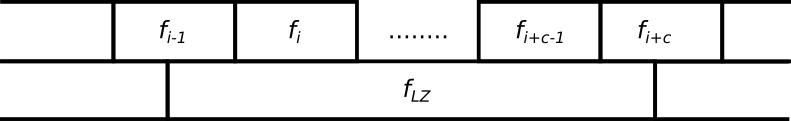
\includegraphics[width=\textwidth,keepaspectratio]{faktorenmerge}
	\caption{Der Faktor $f_{LZ}$ erstreckt sich von $f_{i-1}$ bis $f_{i+c}$}
	\label{flz}
\end{figure}\\
Das bedeutet, dass wir maximal $c$-mal mehr Faktoren in der \textit{c-optimale} LZ-Approximation finden, als in der  LZ-Zerlegung.
Die Anzahl der Faktoren in der Approximation ist also durch die Anzahl der Faktoren in der LZ-Zerlegung multipliziert mit $c$ nach oben beschränkt.  
\begin{equation}
\rho = max
\left\{
\frac{c*f(s_{opt})}{f(s_{opt})},\frac{f(s_{opt})}{c * f(s_{opt})}
\right\}
\end{equation}
\begin{equation}
\rho = c
\end{equation}
Aus einer \textit{c-Optimalität} der Approximation folgt eine Güte der Approximation von $c$ \cite{LZ77Approx}.
%
%
%
\newpage
%
%
%
\section{Hashfuntionen}

Eine \emph{Hashfunktion} $h$ ist eine polstellenlose  Funktion von einem \emph{Universum U} auf eine beschränkte Teilmenge der natürlichen Zahlen $h:U \rightarrow \{0,1,2\cdots ,n \}$.
Die Eingaben bezeichnet man als Schlüssel und die Ausgaben als Hashcodes, eine Hashfunktion definiert  damit \emph{key value pairs}.
Wenn unterschiedliche Schlüssel den gleichen Hashcode besitzen, bezeichnet man dies als \emph{Kollision}.
Wenn die Menge der Eingaben größer ist als die Menge der Hashcodes, sind diese unvermeidlich.\\
Zwei Arten von Hashfunktionen  haben sich für den üblichen Gebrauch durchgesetzt, die Modulo- und die Multiplikationmethode.\\
Hashfuntionen der Modulomethode haben die Form $h(x)=x \  mod \  M$.
Hashfuntionen der Multiplikationmethode besitzen die Form $h(x)= \lfloor M * (x * A \ mod 1) \rfloor $ mit $0<A<1$.\\
$M$ ist meist eine Primzahl um eine möglichst gleiche Verteilung der Hashcodes zu erzielen.
Eine Hashfunktion lässt sich an hand folgender zentraler Kriterien bewerten:
\begin{enum}
	\item Gleichverteilung: alle Hashcodes sollen mit möglich gleicher Wahrscheinlichkeit getroffen werden
	\item Deterministisch: immer gleiche ergebinnie
\end{enum}
	
\section{Fingerprint und rolling Hash}

Ein \emph{Fingerprint} ist der Hashcode der einem String zugeordnet wird.
Fingerprints erlauben es Strings schneller zu vergleichen. 
Um herauszufinden ob zwei Strings $s_{1},s_{2}$ gleich sind müssen wir alle Symbole miteinander vergleichen.
Sollten die beiden Strings sich nur im letzten Symbol unterscheiden so haben wir alle vorherigen Symbole umsonst überprüft.
Vergleichen wir aber vorher beide Fingerprints können wir nicht gleiche Strings direkt erkennen, dies ist wesentlich effizienter da Fingerprints meist deutlich kürzer sind als die Strings selber.
Es kann aber sein, dass durch eine Kollision unterschiedliche Strings den gleichen Fingerprint besitzen.
Daher nicht aus nur die Fingerprints zu vergleichen um zusagen das zwei Strings gleich sind.
Wenn die Fingerprints gleich sind müssen danach alle Symbole des Strings untersucht werden.




Eine Hashtabelle ist eine Liste, in der jeder Hashcode einem Index entspricht.
Die zugehörige Datenstruktur ist die \emph{Hashtabelle}.


	% Literaturverzeichnis
	\bibliographystyle{gerplain}
	\bibliography{diplom}
	\addcontentsline{toc}{chapter}{\bibname}
	
\end{document}
